\documentclass[11pt]{article}
%\usepackage[margin=1.7cm,top=2.5cm,bottom=2.5cm,letterpaper]{geometry}
\usepackage[margin=1cm,top=1.5cm,bottom=1.5cm,papersize={8.5in,17in}]{geometry}
\usepackage{enumitem}
\usepackage{tikz,graphicx,wrapfig}
\usepackage{pgfplots}
\usepackage{amsmath}
\usepackage{newtxtext,newtxmath}
\usepackage[document]{ragged2e}
\usepackage[none]{hyphenat}
\usepackage{siunitx}
\usepackage{multicol}
\usepackage{fancyhdr}

\renewcommand{\headrulewidth}{0pt}

\pagestyle{fancy}
\rhead{}
\chead{}
\lhead{}
%\lfoot{}\cfoot{-\textsf{\textbf{\thepage}}-}
%\rfoot{\textsf{\textbf{GO ON TO THE NEXT PAGE.}}}
\lfoot{}
\rfoot{}

\newcommand{\pic}[2]{
  \begin{center}\includegraphics[width=#1\textwidth]{#2}\end{center}
}
\newcommand{\mb}[1]{\ensuremath\mathbf{#1}}
\sisetup{
  detect-all,
  inter-unit-product =\ensuremath{\cdot},
  per-mode=symbol
}
\tikzset{>=latex}

\begin{document}

\begin{center}
  \textbf{PHYSICS 1\\
    Section II\\
    Time--1 hour 30 minutes\\
    5 Questions
  }
\end{center}

\textbf{Directions:} Questions 2 and 3 are short free-response questions
that require about 13 minutes each to answer and are worth 7 points each.
Questions 1 is a long free-response question that require about 25
minutes each to answer and are worth 12 points. Show your work for each
part in the space provided after that part.

\pic{.4}{swing-around}
\begin{enumerate}
\item A small sphere of mass $M$ is suspended by a string of length $L$. The
  sphere is made to move in a horizontal circle of radius $R$ at a constant
  speed, as shown above. The center of the circle is labeled point $C$, and the
  string makes an $\theta_0$ with the vertical.
  \begin{enumerate}
  \item Two students are discussing the motion of the sphere and make the
    following statements.
    
    \vspace{.1in}Student 1: None of the forces exerted on the sphere are in the
    direction of point $C$, the center of the circular path. Therefore, I don't
    see how there can be a centripetal force exerted on the sphere to make it
    move in a circle.

    \vspace{.1in}Student 2: I see another problem. The tension force exerted by
    the string is at an angle from the vertical. Therefore, its vertical
    component must be less than the weight $Mg$ of the sphere. That means the
    net force on the sphere has a downward vertical component, and the sphere
    should move downward as well as moving around in a circle.

    \vspace{.1in}\begin{enumerate}
    \item What is one aspect of Student 1's reasoning that is incorrect?
    \item What is one aspect of Student 2's reasoning that is incorrect?
    \end{enumerate}
    
  \item
    \begin{enumerate}
    \item Derive an equation for the magnitude of the net force exerted on
      the sphere. Express your answer in terms of $M$, $\theta$, and physical
      constants, as appropriate.
    \item Describe one aspect or step in your derivation of part (b)(i) that
      can be correctly linked to your answer to either part (a)(i) or part
      (a)(ii).
    \end{enumerate}
  \end{enumerate}
  \newpage

  \pic{.3}{swing-backandforth}
  Instead of moving in a horizontal circle, the sphere now moves in a vertical
  plane so that it is a simple pendulum, as shown above. The maximum angle
  $\theta_\mathrm{max}$ that the string makes from the vertical can be assumed
  to be small. The graph below shows data for the square of the pendulum period
  $T$ as a function of string length $L$.

  \pic{.5}{T2-L}
  \begin{enumerate}[resume]
  \item On the graph above, draw a best-fit line for the data. Then use the
    line to calculate a numerical value for the gravitational acceleration $g$.
    \newpage

    \begin{center}
      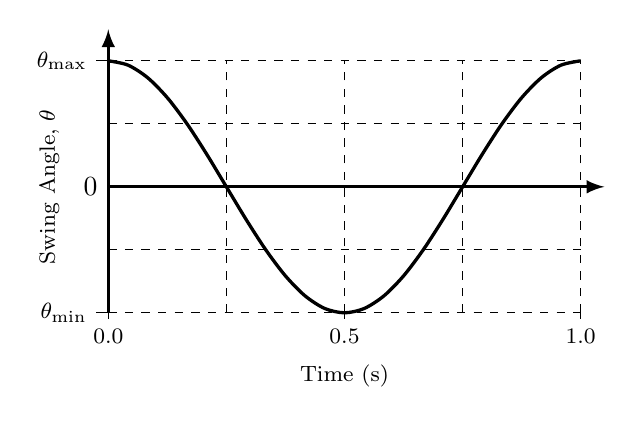
\begin{tikzpicture}[xscale=1.5,yscale=.8]
        \draw[->,very thick](0,0)--(4.2,0) node[pos=0,left]{0};
        \draw[->,very thick](0,-2)--(0,2.5);
        \draw[dashed,thin](0,-2) grid(4,2);
        \draw[domain=0:4,smooth,very thick] plot({\x},{2*cos(90*\x)});
        \draw(0,2)--(-.1,2)node[left]{\footnotesize $\theta_\text{max}$};
        \draw(0,-2)--(-.1,-2)node[left]{\footnotesize $\theta_\text{min}$};
        \node at (2,-3) {\footnotesize Time (s)};
        \foreach\x in {0.0,0.5,1.0}{
          \draw(4*\x,-2)--(4*\x,-2.1) node[below]{\footnotesize \x};
        }
        \node[rotate=90] at (-.5,0) {\footnotesize Swing Angle, $\theta$};
      \end{tikzpicture}
    \end{center}
  \item The graph above shows the angle $\theta$ from the vertical as a function
    of time for the pendulum. On the axes below, sketch a graph of the
    gravitational potential energy of the sphere-Earth system for the same time
    interval. Take the zero of potential energy to be when the potential energy
    has its a minimum value.
    \begin{center}
      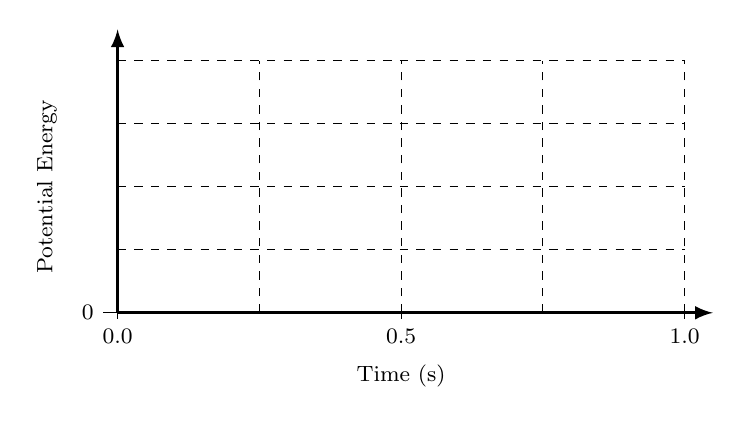
\begin{tikzpicture}[xscale=1.8,yscale=.8]
        \draw[->,very thick](0,-2)--(4.2,-2);
        \draw[->,very thick](0,-2)--(0,2.5);
        \draw[dashed,thin](0,-2) grid(4,2);
        \node at (2,-3) {\footnotesize Time (s)};
        \draw(0,-2)--(-.1,-2) node[left]{\footnotesize 0};
        \foreach\x in {0.0,0.5,1.0}{
          \draw(4*\x,-2)--(4*\x,-2.1) node[below]{\footnotesize \x};
        }
        \node[rotate=90] at (-.5,0) {\footnotesize Potential Energy};
      \end{tikzpicture}
    \end{center}
  \item As the sphere swings back and forth, it must also rotate a small amount
    during each swing. The figures below indicate the direction that the sphere
    rotates as it is swinging in each direction.
    \pic{.5}{swings}
    In order for the sphere's rotation to change direction, a torque must be
    exerted on the sphere. When the sphere is at its maximum rightward
    displacement, what is the direction of the torque exerted on the sphere
    with respect to the point of attachment between the sphere and string?

    \vspace{.1in}
    \underline{\hspace{.3in}} Clockwise\hspace{.3in}
    \underline{\hspace{.3in}} Counterclockwise
        
    \vspace{.1in}Briefly state why the torque is in the direction you indicated.
  \end{enumerate}
  \newpage

  \pic{.4}{masses-and-springs}  
\item A spring with unstretched length $L_1$ is hung vertically, with the top
  end fixed in place, as shown in Figure 1 above. A block of mass $M$ is
  attached to the bottom of the spring, as shown in Figure 2, and the spring
  has length $L_2>L_1$ when the block hangs at rest. The block is then pulled
  downward and held in place so that the spring is stretched to a length
  $L_3>L_2$, as shown in Figure 3.
  \begin{enumerate}[leftmargin=18pt]
  \item On the dot below, which represents the block in Figure 3, draw and
    label the forces (not components) exerted on the block. Each force must be
    represented by a distinct arrow starting on, and pointing away from, the
    dot.
    
    \vspace{.7in}
    \begin{center}
      {\tikz\fill(0,0)circle(.2);}
    \end{center}
    \vspace{.7in}

  \item The student releases the block. Consider the time during which the
    block is moving upward toward its equilibrium position and the spring
    length is still longer than $L_2$. In a clear, coherent paragraph-length
    response that may also contain diagrams and/or equations, indicate why the
    total mechanical energy is increasing, decreasing, or constant for each of
    the systems listed below.
    \begin{itemize}
    \item System 1: The block
    \item System 2: The block and the spring
    \item System 3: The block, the spring, and Earth
    \end{itemize}
    Use $E_1$, $E_2$, and $E_3$ to denote the total mechanical energy of
    systems 1, 2, and 3, respectively.
  \end{enumerate}
  \newpage

  \pic{.8}{tuning-fork}
\item To demonstrate standing waves, one end of a string is attached to a
  tuning fork with frequency \SI{120}{\hertz}. The other end of the string
  passes over a pulley and is connected to a suspended mass $M$ as shown in the
  figure above. The value of $M$ is such that we standing wave pattern has four
  ``loops''. The length of the string from the tuning fork to the point where
  the string touches the top of the pulley is 1.20 m. The linear mass density
  of the string is \SI{1.e-4}{\kilo\gram\per\metre}, and remains constant
  throughout the experiment.
  \begin{enumerate}
  \item Determine the wavelength of the standing wave.
  \item Determine the speed of the transverse waves along the string.
  \item The speed of waves along the string increases with increase tension in
    the string. Indicate whether the value of $M$ should be increases or
    decreased in order to double the number of loops in the standing wave
    pattern. Justify your answer.
  \item If a point on the string at an antinode moves a total vertical distance
    of 4 cm during one complete cycle, what is the amplitude of the standing
    wave?
  \end{enumerate}
\end{enumerate}
\end{document}
